% !TeX root = ../../../main.tex

% Key observations:
% - direction of change in PD and RE/RV are opposite here, too
% - RE and RV also appear incredibly similar in trends, just like DoA
% - PD, RE, and RV-based DoA are all significantly different in:
%   - IFTA 0 vs 2: outer medulla vs inner medulla
%   - i-IFTA 0 vs 2: outer medulla vs inner medulla
%   - Rejection: outer/inner cortex, outer/inner medulla

\begin{figure}[!tbp]
    \centering
    \begin{subfigure}[b]{\textwidth}
        \centering
        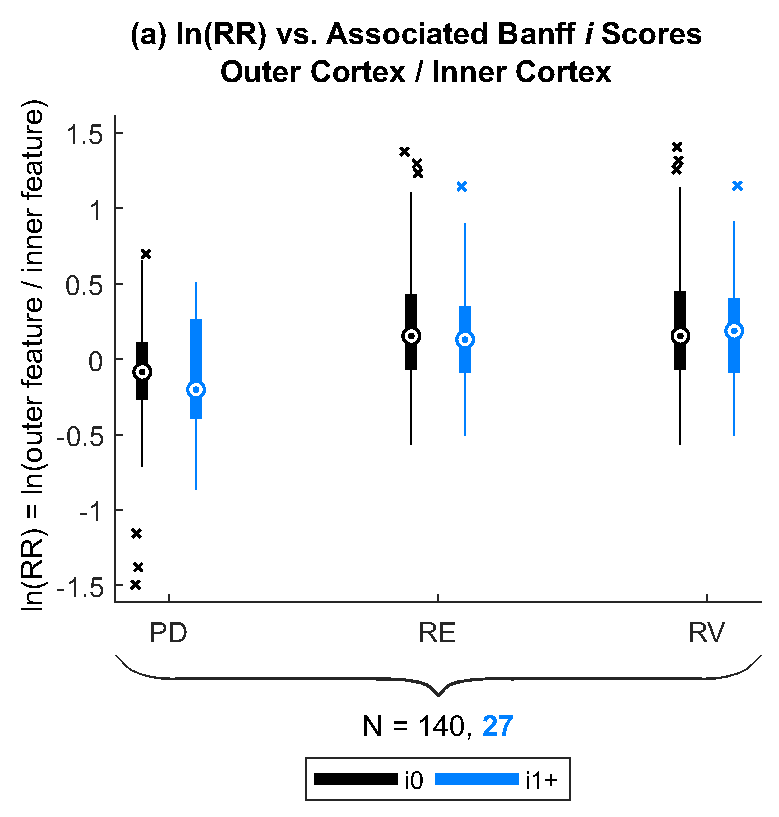
\includegraphics[width=0.24\textwidth]{
            parts/transplant/figs/boxplot-rr/rr-all-i/rr_F1.5_i_oc-ic.eps
        }
        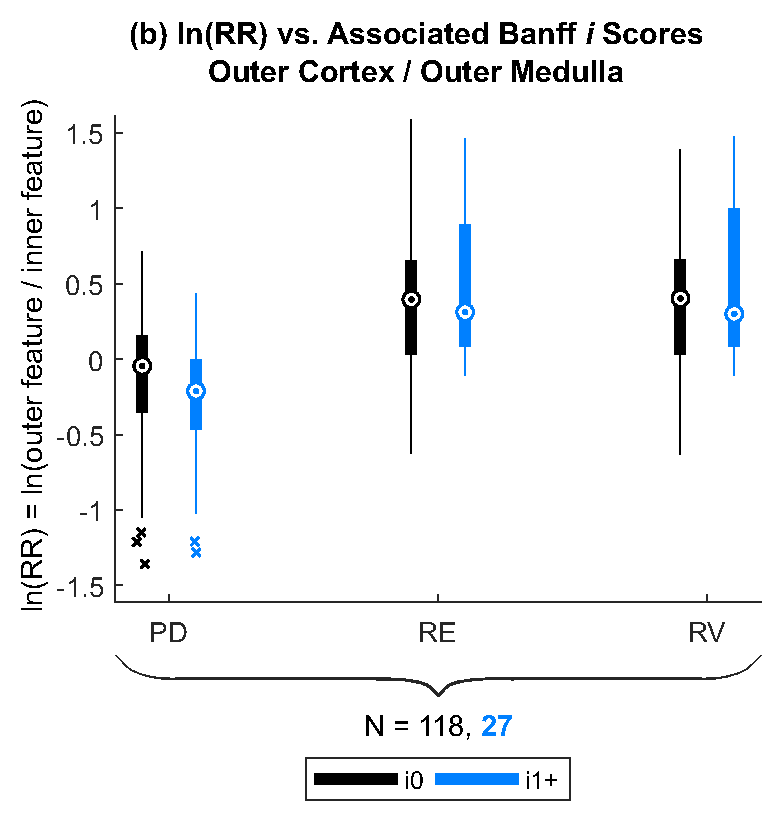
\includegraphics[width=0.24\textwidth]{
            parts/transplant/figs/boxplot-rr/rr-all-i/rr_F1.5_i_oc-om.eps
        }
        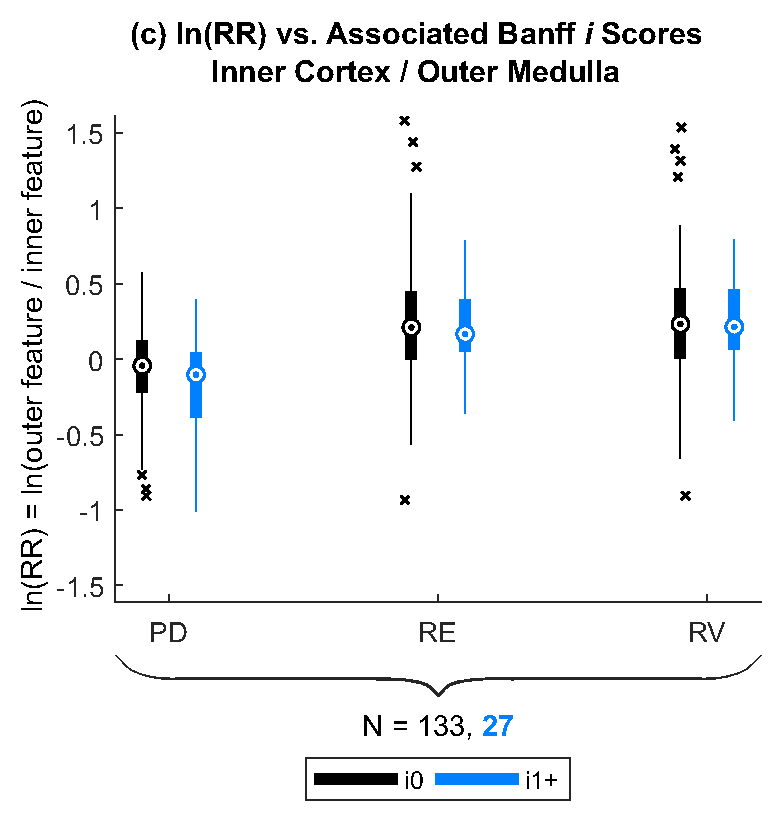
\includegraphics[width=0.24\textwidth]{
            parts/transplant/figs/boxplot-rr/rr-all-i/rr_F1.5_i_ic-om.eps
        }
        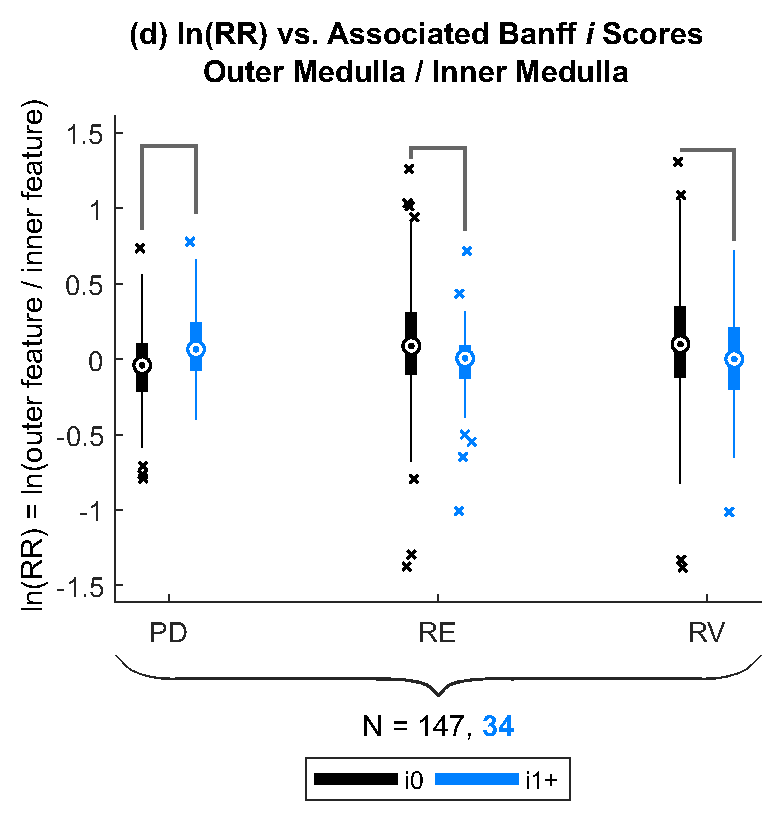
\includegraphics[width=0.24\textwidth]{
            parts/transplant/figs/boxplot-rr/rr-all-i/rr_F1.5_i_om-im.eps
        }
    \end{subfigure}
    \begin{subfigure}[b]{\textwidth}
        \centering
        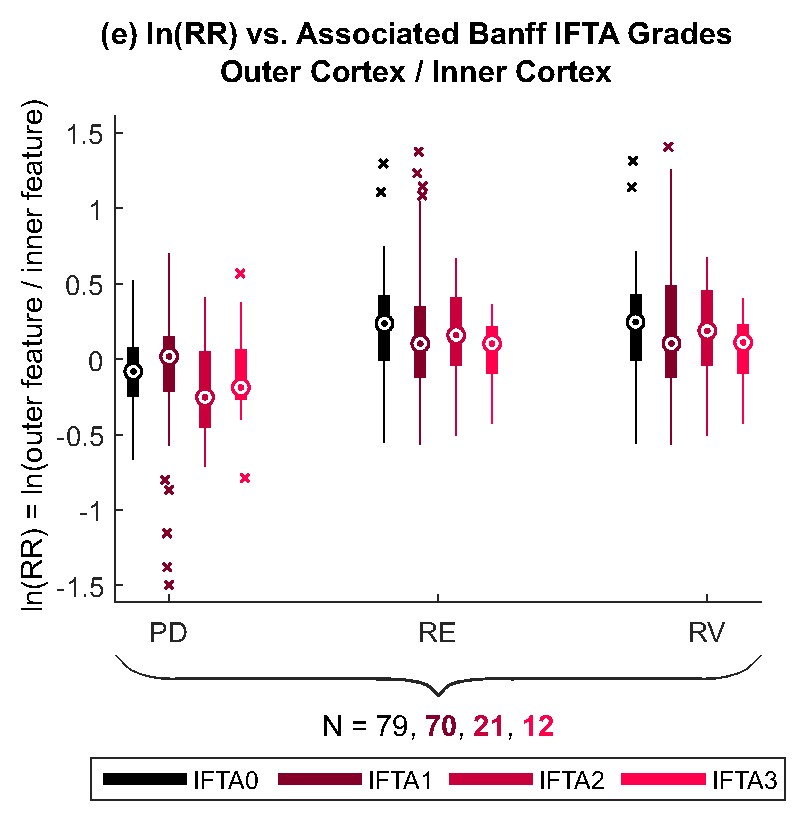
\includegraphics[width=0.24\textwidth]{
            parts/transplant/figs/boxplot-rr/rr-all-ifta/rr_F1.5_ifta_oc-ic.eps
        }
        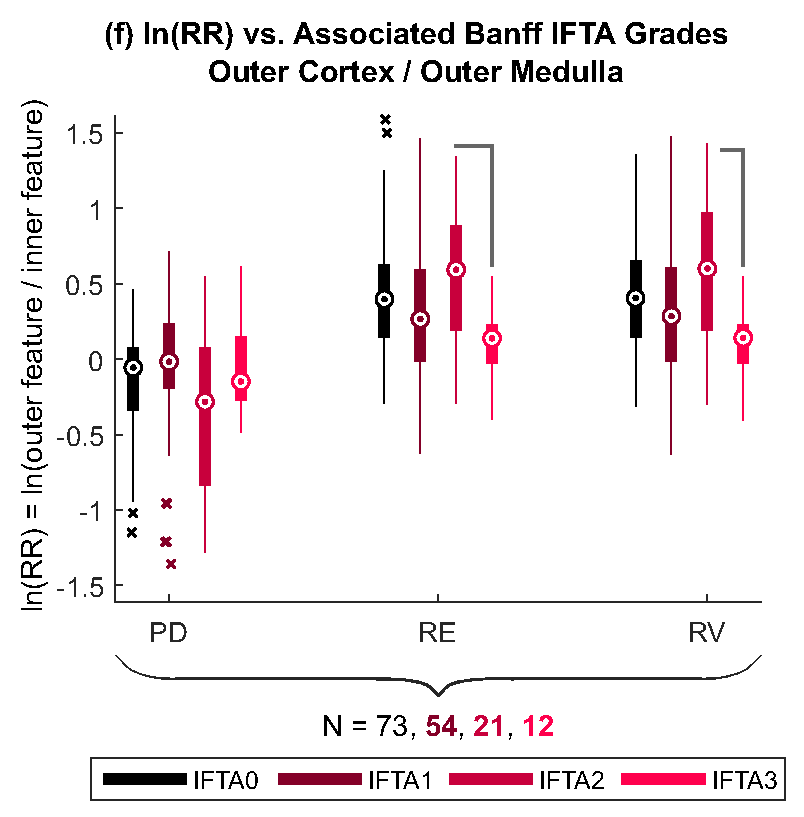
\includegraphics[width=0.24\textwidth]{
            parts/transplant/figs/boxplot-rr/rr-all-ifta/rr_F1.5_ifta_oc-om.eps
        }
        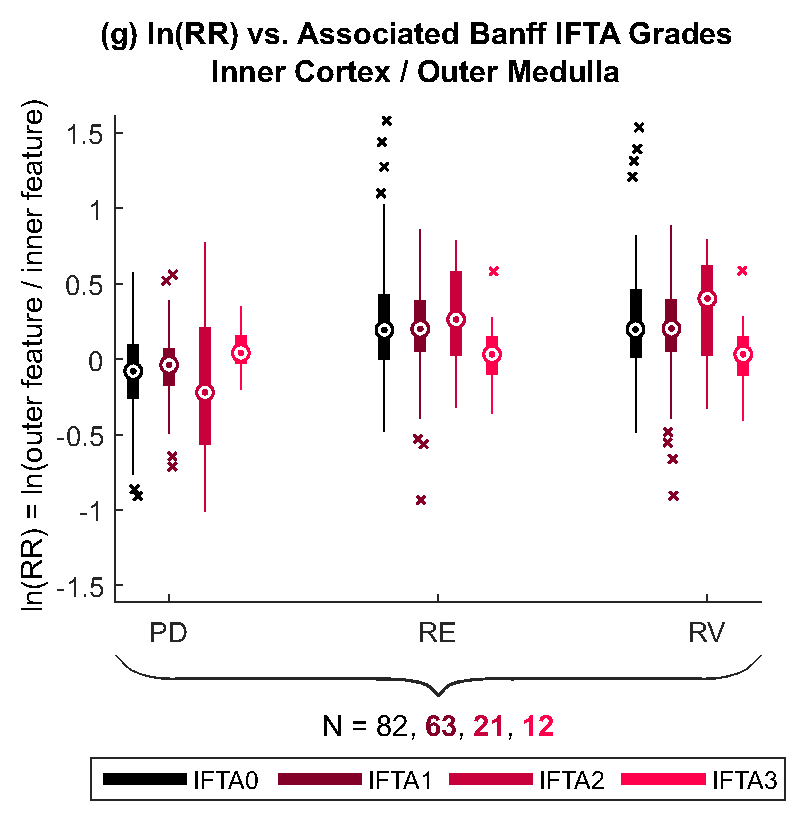
\includegraphics[width=0.24\textwidth]{
            parts/transplant/figs/boxplot-rr/rr-all-ifta/rr_F1.5_ifta_ic-om.eps
        }
        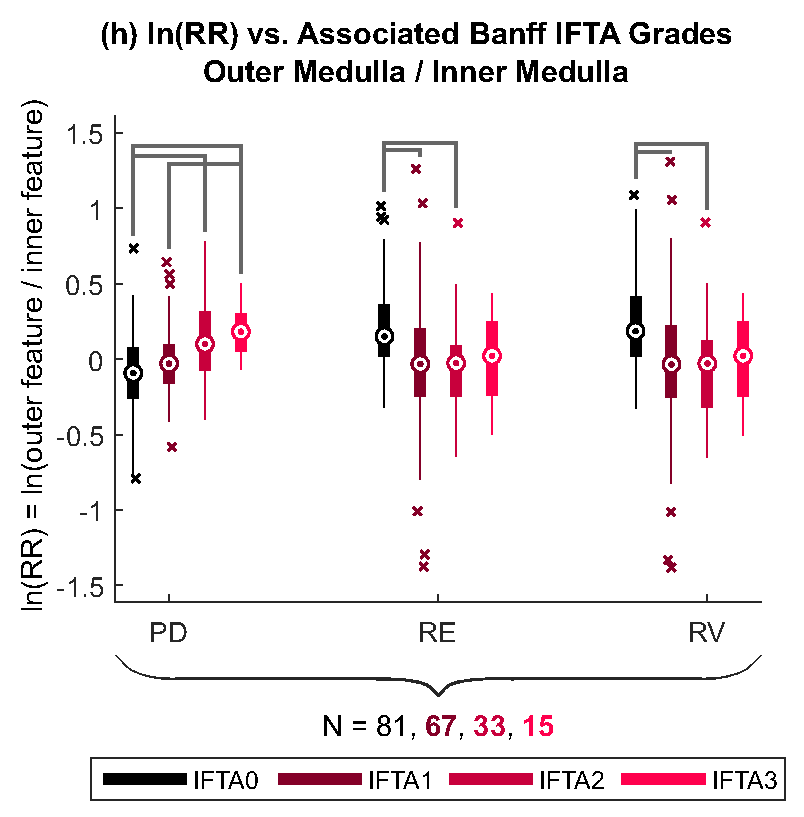
\includegraphics[width=0.24\textwidth]{
            parts/transplant/figs/boxplot-rr/rr-all-ifta/rr_F1.5_ifta_om-im.eps
        }
    \end{subfigure}
    \begin{subfigure}[b]{\textwidth}
        \centering
        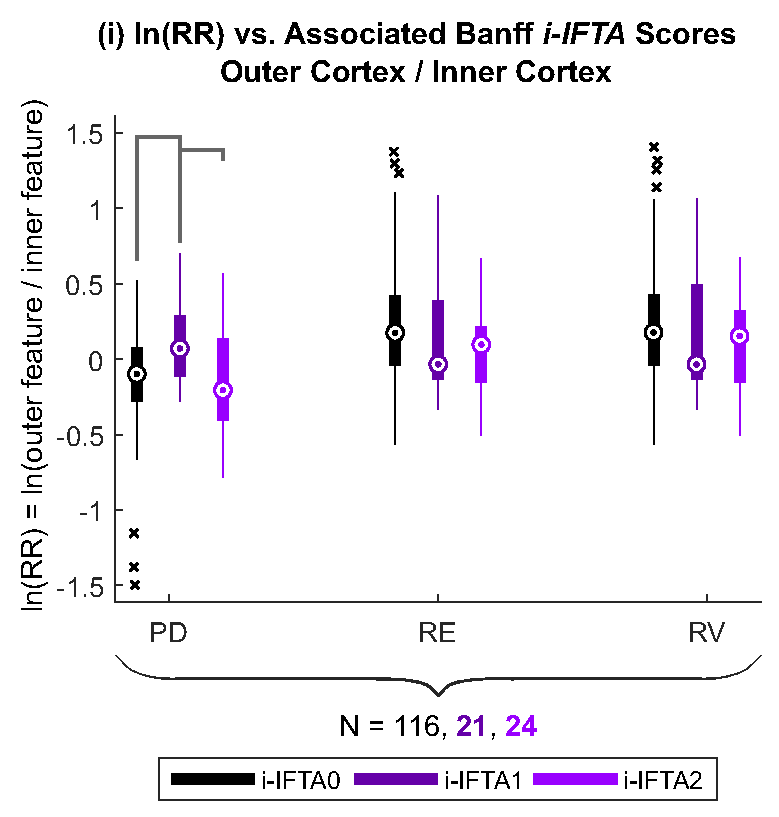
\includegraphics[width=0.24\textwidth]{
            parts/transplant/figs/boxplot-rr/rr-all-i-ifta/rr_F1.5_i-ifta_oc-ic.eps
        }
        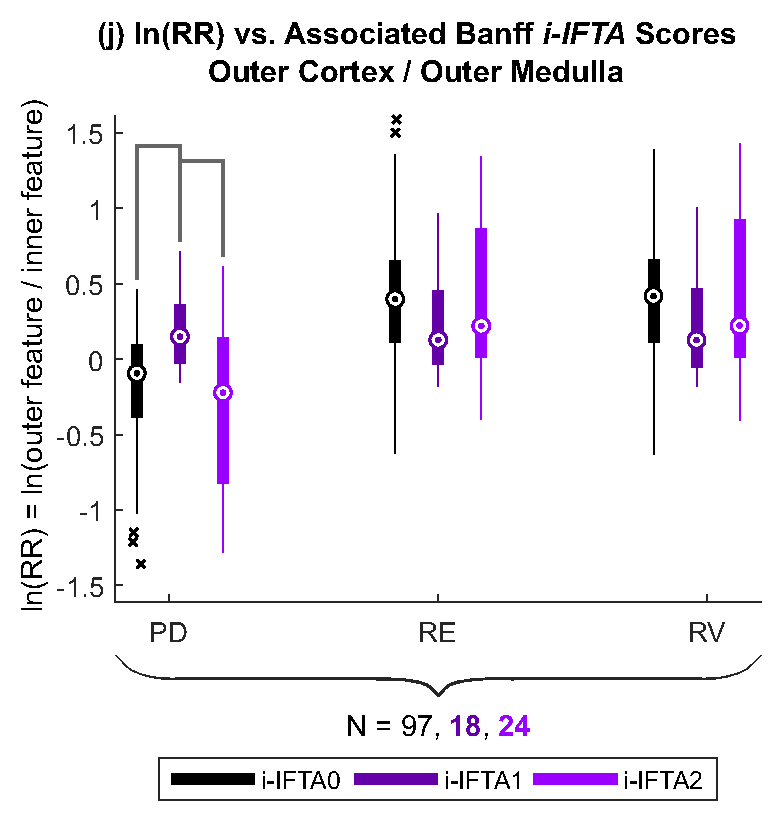
\includegraphics[width=0.24\textwidth]{
            parts/transplant/figs/boxplot-rr/rr-all-i-ifta/rr_F1.5_i-ifta_oc-om.eps
        }
        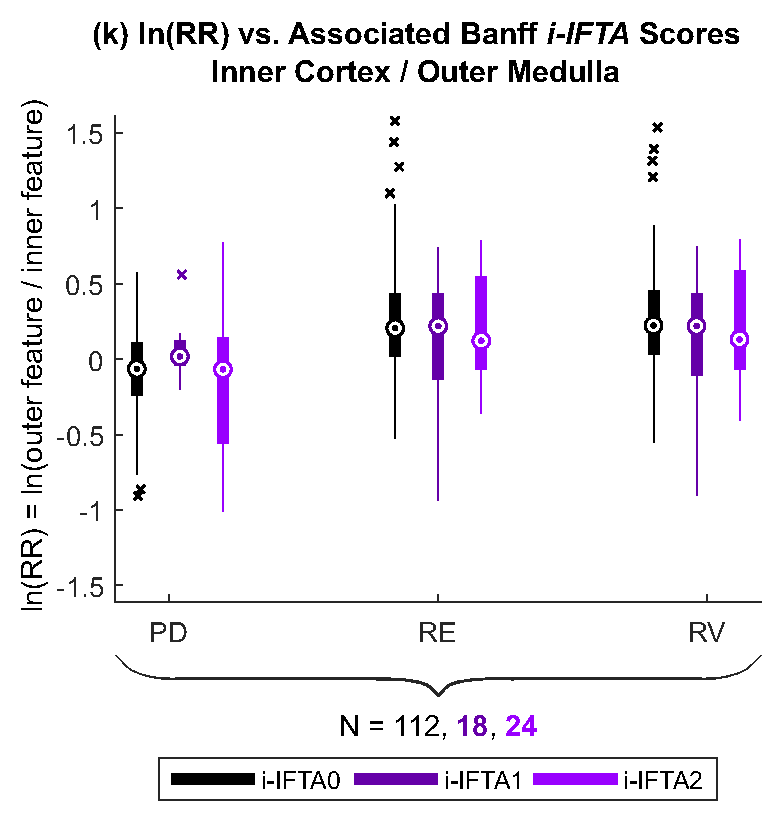
\includegraphics[width=0.24\textwidth]{
            parts/transplant/figs/boxplot-rr/rr-all-i-ifta/rr_F1.5_i-ifta_ic-om.eps
        }
        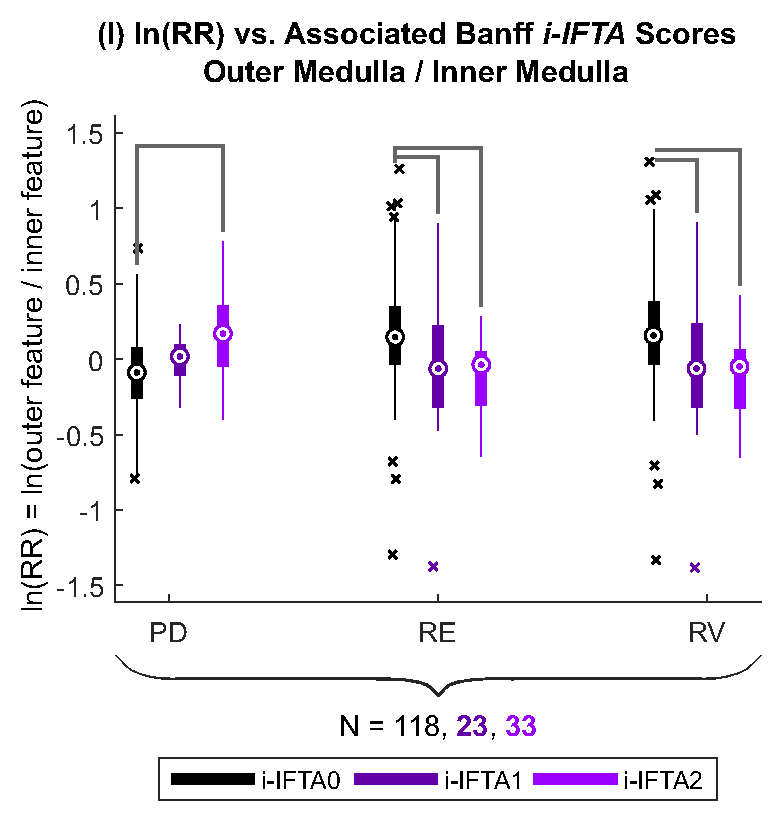
\includegraphics[width=0.24\textwidth]{
            parts/transplant/figs/boxplot-rr/rr-all-i-ifta/rr_F1.5_i-ifta_om-im.eps
        }
    \end{subfigure}
    \begin{subfigure}[b]{\textwidth}
        \centering
        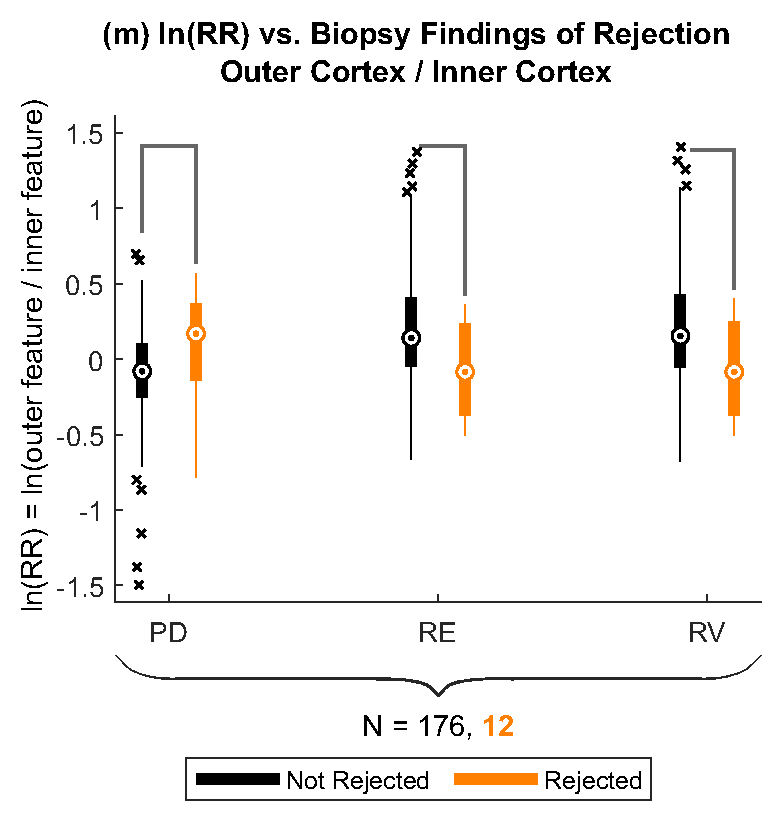
\includegraphics[width=0.24\textwidth]{
            parts/transplant/figs/boxplot-rr/rr-all-reject/rr_F1.5_reject_oc-ic.eps
        }
        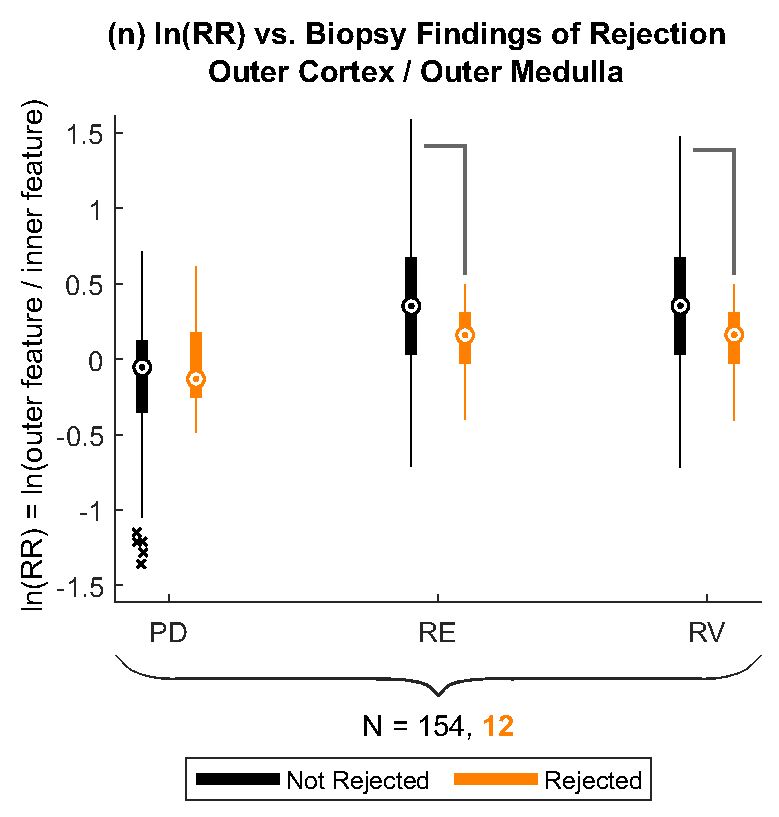
\includegraphics[width=0.24\textwidth]{
            parts/transplant/figs/boxplot-rr/rr-all-reject/rr_F1.5_reject_oc-om.eps
        }
        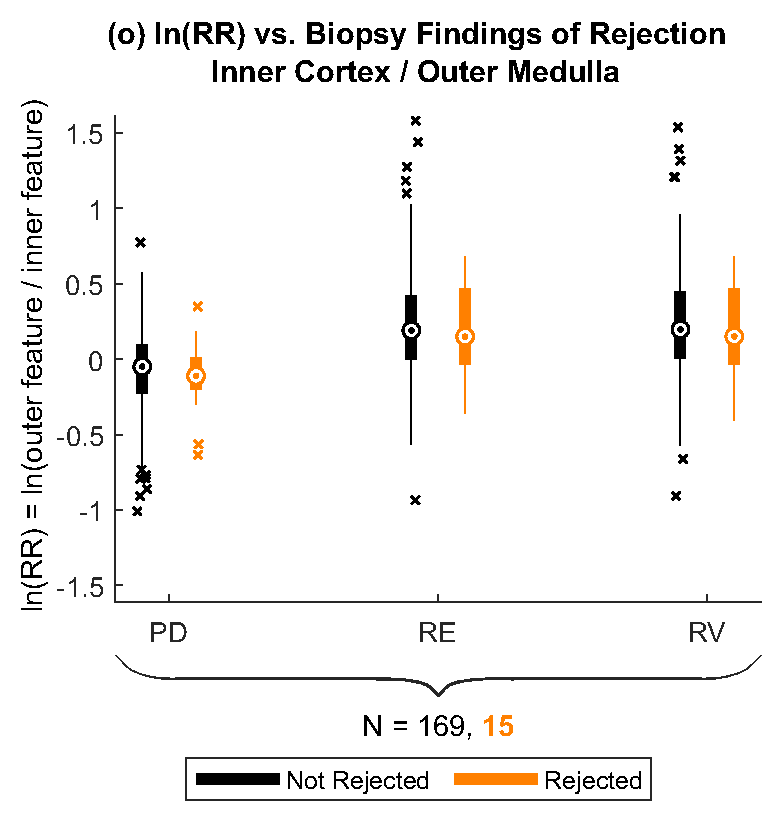
\includegraphics[width=0.24\textwidth]{
            parts/transplant/figs/boxplot-rr/rr-all-reject/rr_F1.5_reject_ic-om.eps
        }
        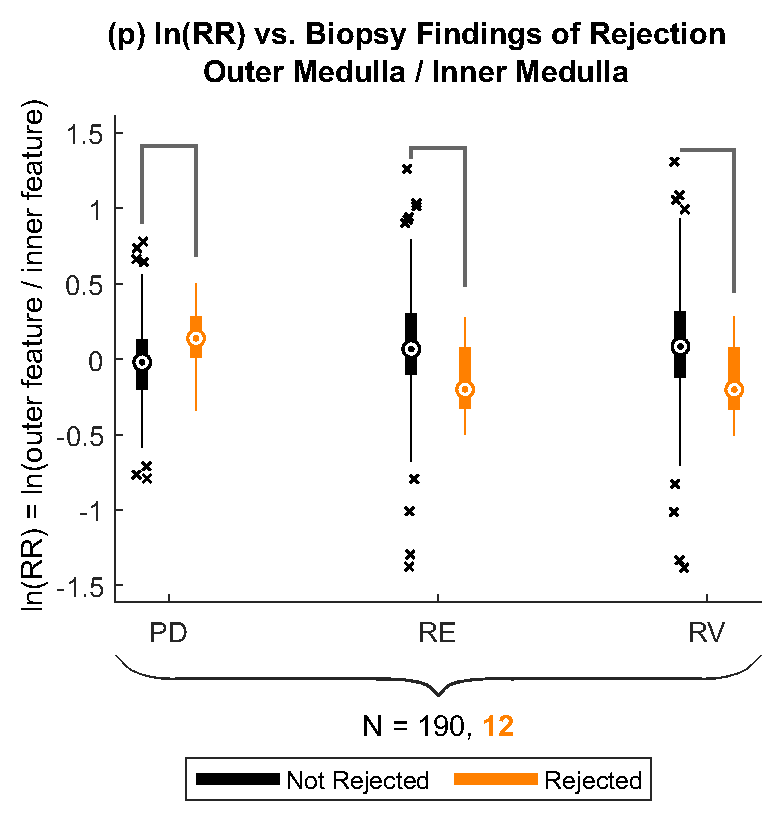
\includegraphics[width=0.24\textwidth]{
            parts/transplant/figs/boxplot-rr/rr-all-reject/rr_F1.5_reject_om-im.eps
        }
    \end{subfigure}
    \caption{Box plots of RR based on PD, RE, and RV measurements, grouped by associated biopsy findings of (a--d) \emph{i} (interstitial inflammation) scores, (e--h) IFTA (interstitial fibrosis/tubular atrophy) grading, (i--l) \emph{i-IFTA} (inflammation in areas of IFTA) scores, and (m--p) whether biopsies indicated graft rejection. Values are shown for RR between the (a,e,i,m) outer versus inner cortex, (b,f,j,n) outer cortex over outer medulla, (c,g,k,o) inner cortex over outer medulla, and (d,h,l,p) outer versus inner medulla. Numbers written under x-axes denote number of ROIs represented by each distribution. Pairs of box plots connected with gray bars denote statistically significant differences ($p < 0.05$) between biopsy findings based on Kruskal-Wallis test and Bonferroni correction. RR values without matched biopsy findings are not shown.}
    \label{fig:clinicalVisrRr}
\end{figure}
